

\chapter{Distributed GPU SpMV}
\label{chap:multigpu_rbffd}

%%%%%%%%%%

%DONE: extending work from chapter 6 we return to the GPU but this time attempt to span multiple GPUs
%TODO: describe context with multiple devices, we assume one device per context
%TODO: describe multiple queues, assume two for SpMV (why? indep operation, overlapping kernel execution not just comm)
%TODO: nonoverlapping test case description
%TODO: overlapping test case description
%TODO: benchmark nonoverlapping shows significant loss on multiple GPUs one host
%TODO: Known issue on Cascade is that all GPUs are attached to the same I/O hub
%TODO: limits performance because transfers to each GPU are serialized 
%TODO: we have explicit barrier on comm ensuring that each kernel gets to transfer at the same time
%TODO: benchmark overlapping shows 5x boost because queues do not necessarily transfer at the same time
%TODO: also the multiple queues ensure overlapping memtransfer and some comp with the original spmv. 
%TODO: a single queue would have synchronous copy following kernel execution and synchronous SpMV if both in same queue
%TODO: two queues allows asynchronous copy and overlap between SpMVs.

%TODO: cuda mpi aware


Today, high performance computing centers around the world are leveraging GPU accelerators to reach their peak performance. For example, the Titan supercomputer at Oak Ridge National Lab is (as of this writing) ranked \#2 on the world-wide Top500 list, and achieved that spot with a total of 18,688 NVidia K20 GPUs and 18,688 AMD Opteron CPUs in a 1:1 pairing for a theoretical peak of 27.1 PFLOP/sec \cite{TitanGPUCluster}. 
In some cases, HPC installations like the Keeneland project \cite{Vetter2011} boast significantly more GPU accelerators than CPU counterparts. The Keeneland Full-Scale (KFS) system has 528 Intel Sandy-Bridge CPUs and 792 NVidia Fermi-class GPUs in 264 compute nodes (i.e., 2:3 CPUs:GPUs), and a theoretical peak of 615 TFLOP/sec \cite{Vetter2011}. 

Ultimately, finding a way to harness the tera- and peta-scale performance from such clusters is a grand challenge for our work on RBF-FD and other RBF PDE methods. To this end, we present a multi-GPU implementation of RBF-FD.

In Chapter~\ref{chap:gpu_rbffd}, we have already developed two different approaches to computing RBF-FD on a single GPU: the first using custom OpenCL kernels for RK4 time-steps, and the second using ViennaCL for the same tasks. Then in Chapter~\ref{chap:distributed_rbffd}, we laid the foundation for a distributed RBF-FD that spans the nodes of an HPC cluster, and demonstrated scaling up to 1024 processors (128 nodes). This chapter combines those algorithms to produce the first (to our knowledge) multi-GPU implementation of the RBF-FD method with overlapping communication and computation. 

One issue with distributing computation across multiple GPUs is that the GPUs excel at accelerating computation, but do nothing to reduce the cost of communication. With communication latency suddenly disproportionately large compared to computation, the distributed GPU implementation loses its ability to scale well. As part of this chapter, we detail an algorithm to hide communication latency behind overlapped computation. The algorithm presented herein is an organic extension to the overlapping communication and computation algorithm in Chapter~\ref{chap:distributed_rbffd}. 

Our multi-GPU implementation leverages non-blocking MPI communication plus two asynchronous OpenCL queues to amortize the cost of data transfer between CPU and GPU, MPI communication, and in some cases hide some computation. 

%With the popularity of GPU clusters, there are naturally a number of related investigations in the literature that consider overlapping communication and computation for multi-GPU applications. For example, Kim and Park overlap communication and computation in their implementation of a Finite-Difference Time-Domain algorithm and demonstrate near perfect strong scaling up to 6 GPUs \cite{KimPark2012}. \cite{Thibault2009}
%
%TODO: \cite{Goeddeke2009} \cite{Erez2007}
%Similar approaches to overlapping communication and computation can be found in \cite{Schubert2011} and \cite{Thibault2009}.

%Lawlor \cite{Lawlor2009} wraps a subset of MPI collectives, memory copies between GPU and CPU, and---to some extent---callbacks to GPU kernels behind a simplified API called cudaMPI. Although the concept of cudaMPI is good for minimally invasive design, the library only provides a handful of  a limited subset of MPI  a for overlapping communication and computation.  


\section{Multi-GPU RBF-FD}

In order to develop the multi-GPU implementation, we return to the idealized test case proposed in Chapter~\ref{chap:distributed_rbffd}: four derivatives on a 3-D regular grid are computed via SpMV and used as the intermediate vectors for an RK4 time-step. At the end of each SpMV a communication collective synchronizes external dependencies for each subdomain.

In Chapter~\ref{chap:distributed_rbffd}, the SpMV was assumed run on the CPU. Herein, it is assumed to be computed via one of the GPU algorithms presented in Chapter~\ref{chap:gpu_rbffd}. For now the actual choice between custom OpenCL kernels and ViennaCL does not matter. Later, when we consider the scaling of this algorithm, the ViennaCL implementation is assumed. 

Our original attempt at multi-GPU RBF-FD, described in \cite{BolligFlyerErlebacher2012}, utilized blocking communication (i.e., \texttt{MPI\_Send}/\texttt{MPI\_Recv}) for synchronization. The blocking communication functioned for debugging purposes, but was not practical. In Appendix~\ref{app:keeneland_alltoallv_benchmarks}, we provide supplementary data that demonstrates the result of replacing the blocking send and receives with an \texttt{MPI\_Alltoallv} (i.e., the GPU equivalent of Figure~\ref{fig:alltoallv_cpu}). In both cases the SpMV is a single kernel launch and the synchronization includes both an encode and decode phase (see \S~\ref{sec:local_ordering}). 

The two multi-GPU algorithms presented in this chapter build on Figure~\ref{fig:no_decode_cpu} and Figure~\ref{fig:overlap_cpu}; the final collectives tested in \S~\ref{sec:mpi_improvements}. 

Figure~\ref{fig:isendirecv_gpu} presents 

   \begin{enumerate}
    \item Transfer $\mathcal{O}$ from GPU to CPU
    \item Encode $\mathcal{O}$ to send buffer
	\item Distribute $\mathcal{O}$ to other CPUs and receive $R$ from other CPUs
	\item Decode $\mathcal{R}$ from received buffer  
	\item Transfer $\mathcal{R}$ to the GPU
	\item Launch a GPU kernel to operate on $\mathcal{Q}$
   \end{enumerate} 

When operating on multiple GPUs we avoid the copy-out or decode phase by requiring that the local ordering of nodes sort the set $\setDepend$ by the rank of the process sending each node. This way, when the MPI collective finishes and all values arrive contiguous by provider, the data can be copied directly to the GPU without reordering.

\subsection{Overlapping with the GPU}

Overlapping communication and GPU computation is enabled by two levels of asynchronous commands: 
\begin{itemize} 
\item \emph{Non-blocking MPI}. The MPI\_Isend/MPI\_Irecv routines are used to post communication and immediately return the main thread to computation. 
\item \emph{Asynchronous GPU Queues}. Two OpenCL queues are utilized to send commands to the GPU. 
\end{itemize}



Figure~\ref{fig:overlap_gpu}


In Section~\ref{sec:local_ordering}

OpenCL requires that data be explicitly copied to the CPU. The MPI collectives 



\section{Overlapping Communication}
Internal to every OpenCL application is both a Context and a Queue. The Context 

~\ref{sec:index_mappings}



The overlapping communication is achieved by creating additional queues 


Recent advances in distributed (multi-)GPU computing involve NVidia's GPU Direct technology. GPU Direct allows hardware like the PCI-e bus to directly access memory on the GPU device. CUDA V5.5 adds full support for MPI applications 



\section{Multi-GPU Challenges}

Distributing SpMV across multiple GPUs poses a new problem: as previous mentioned, the data sent and received via MPI collectives must be copied from device to host and vice-versa. To amortize this cost we introduce a novel overlapping algorithm to hide the cost of communication behind the cost of a concurrent SpMV on the GPU. 

 
\begin{figure} 
\centering
\begin{subfigure}{0.48\textwidth}
\centering
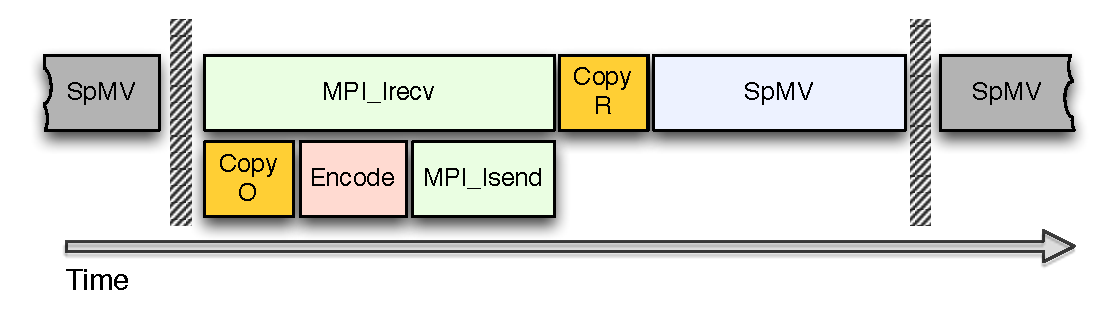
\includegraphics[width=\textwidth]{../figures/omnigraffle/GPU_IsendIrecv.pdf}
\caption{GPU and MPI\_Isend/MPI\_Irecv (Non-Overlapping)}
\label{fig:isendirecv_gpu}
\end{subfigure}
\quad
\begin{subfigure}{0.48\textwidth}
\centering
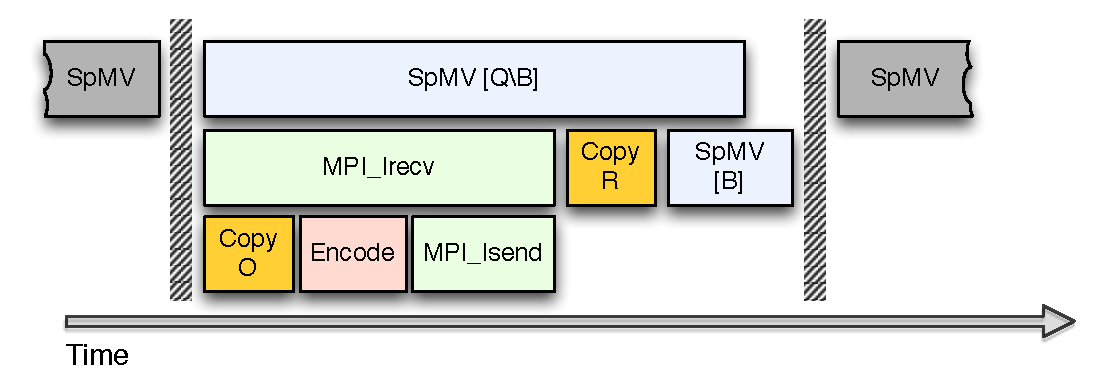
\includegraphics[width=\textwidth]{../figures/omnigraffle/GPU_OverlapGPU.pdf}
\caption{GPU and MPI\_Isend/MPI\_Irecv (Overlapping)}
\label{fig:overlap_gpu}
\end{subfigure}
\caption{Overlapping GPU kernels with CPU managed communication. Task block sizes are not drawn to scale.} 
\label{fig:gpu_mpi_tuning}
\end{figure}


\section{Strong Scaling Performance}

We now consider the performance of our multi-GPU algorithms. 


%Our effort in \cite{BolligFlyerErlebacher2012} developed the original multi-GPU implementation of RBF-FD. 
Appendix~\ref{app:keeneland_alltoallv_benchmarks} presents scaling data for the multi-GPU implementation based on our custom OpenCL kernels that were developed in \cite{BolligFlyerErlebacher2012}. The data was generated on the Keeneland Initial Delivery (KID) system \cite{Vetter2011}. We tested the strong scaling of RBF-FD kernels up to 10 GPUs (1 GPU per compute node) for the small problem size of $N=27556$ nodes. Non-overlapping communication (\texttt{MPI\_Alltoallv}) synchronizes GPUs as they execute iterations of the RK4 time-scheme. The benchmarks on Keeneland tested


In Chapter~\ref{chap:gpu_rbffd} the Cascade GPU cluster was introduced. Recall that Cascade contains up to 32 NVidia M2070 GPUs, 8 NVidia K20 GPUs and 3 Intel Xeon Phis. Although Cascade is not a large GPU cluster, it does present a nice environment for testing scaling 

We scale our ViennaCL ELL format SpMV across the M2070 GPUs on Cascade. This gives us up to 32 GPUs for computation. 

By comparing benchmarks from the non-overlapped and overlapped GPU cases, we get the speedup: 
\begin{align*} 
S_p = \ ^{t_{non-overlapped}} /_{t_{overlapped}}
\end{align*}
in using the overlapped solution. Any reduction in time is evidence of overlap. 

If speedup greater than $p = (Compute Nodes * PPN)$ is achieved 



I/O Hub contention is a known issue on HP ProLiant GPU clusters like Cascade (see e.g., \cite{Spafford2011}). 



In both cases, the performance is based on a non-overlapping communication collective (MPI\_Alltoallv).


\begin{table}[htb]
\centering
\caption{GFLOP/sec achieved by the distributed ELL SpMV on Cascade's M2070 GPUs, with non-overlapping MPI communication. The SpMV computes derivatives over a 3-D regular grid of size $N=4096000$ nodes (i.e., $160^3$). Data reflects various combinations of stencil sizes, number of compute nodes and number of processes per node (PPN). GPUs are attached to each process per node (i.e. 4 PPN implies 4 GPUs). }
\label{tbl:cascade_m2070_nonoverlap}
\begin{tabular}{c|c|c|c|c|c|c}
 \multicolumn{2}{c}{ } & \multicolumn{4}{|c|}{Observed GFLOP/sec} \\  \hline
Compute Nodes   &   PPN  &   n=17   &   n=31   &   n=50   &   n=101   \\ \hline
1  &  1  &  8.4  &  8.4  &  8.9  &   \\
2  &  1  &  6.1  &  6.8  &  6.4  &  7.6 \\
4  &  1  &  6.9  &  9.1  &  10.3  &  13.3 \\
8  &  1  &  12.1  &  14.6  &  12.1  &  23.0 \\ \hline
1  &  2  &  3.4  &  4.1  &  3.7  &  4.2 \\
2  &  2  &  4.4  &  5.4  &  6.5  &  8.1 \\
4  &  2  &  11.1  &  9.3  &  9.9  &  14.2 \\
8  &  2  &  15.9  &  15.4  &  22.2  &  23.9 \\ \hline
1  &  4  &  3.3  &  4.4  &  5.1  &  5.5 \\
2  &  4  &  8.3  &  7.6  &  9.5  &  11.0 \\
4  &  4  &  12.4  &  12.9  &  18.7  &  18.0 \\
8  &  4  &  17.4  &  28.4  &  28.0  &  37.4 
\end{tabular} 
\end{table}


The total time required to compute the distributed SpMV for 1 node and 4 PPN is observed in the neighborhood of 80 ms for $n=50$ and the non-overlapping algorithm (i.e. without splitting $\setCenters \backslash \setBoundary$ and $\setBoundary$). Of those 80 ms, approximately 60 ms is spent performing non-computation tasks such as transferring from GPU down to CPU, encoding and sending data via MPI and then transferring back up to the GPU. The remaining 20 ms is all dedicated to performing the SpMV.

By introducing the overlapped GPU kernels, the total time for the distributed SpMV for $n=50$ (1 node, 4 PPN) drops to approximately 15 ms---25\% less than the SpMV-only portion of the non-overlapped approach. Since the non-computation tasks amount to only 12 ms in the overlapped case, our first conclusion is that overlapping hides 100\% of communication for the cases tested in Table~\ref{tbl:cascade_m2070_overlap}, as well as the entire SpMV for $\setBoundary$. 

Within each block of Table~\ref{tbl:cascade_m2070_overlap} we expect the GFLOP/sec to double by row. Obviously the strong scaling in the case of the GPU is not ideal when executing more than one PPN. However, for $n=50$ and 1 PPN we see super but on only 32 GPUs, and impeded by the I/O hub bottleneck, we manage to achieve 130 GFLOP/sec for $n=101$. Compare this to the GFLOP/sec scaling results on Itasca in Figure~\ref{fig:compare_strong_scaling_gflops_all_stencils} where 130 GFLOP/sec requires approximately 


Greater than 4x speedup (bold-faced in Table~\ref{tbl:cascade_m2070_overlap}) is possible due to a design flaw on Cascade: each compute node has four attached GPUs connected to the host via a shared I/O hub. Concurrent data transfers from multiple GPUs to host, or vice versa---as would occur while executing a synchronized, distributed SpMV---result in contention on the hub and serialization of transfers. Serialization effectively quadruples the total run-time for 4 PPN. By overlapping communication and computation we notice two effects: a) I/O hub contention disappears (or it is at least hidden by computation), and b) 


\begin{table}[htb]
\centering
\caption{GFLOP/sec achieved by the distributed ELL SpMV on Cascade's M2070 GPUs, with MPI communication overlapping two GPU kernels. The SpMV computes derivatives over a 3-D regular grid of size $N=4096000$ nodes (i.e., $160^3$). Data reflects various combinations of stencil sizes, number of compute nodes and number of processes per node (PPN). Quantities in parentheses denote the speedup factors achieved by the overlapping algorithm over the non-overlapping approach for identical combinations of compute nodes, PPN, stencil size, etc. }
\label{tbl:cascade_m2070_overlap}
\begin{tabular}{c|c|c|c|c|c|c}
 \multicolumn{2}{c}{ } & \multicolumn{4}{|c|}{Observed GFLOP/sec (Speedup over Non-overlapped)} \\  \hline
Compute Nodes   &   PPN  &   n=17   &   n=31   &   n=50   &   n=101   \\ \hline
1   &   1   &   8.5 (1.0x)   &   8.4 (1.0x)   &   9.0 (1.0x)   &  --    \\
2   &   1   &   13.8 (2.3x)   &   13.0 (1.9x)   &   13.1 (2.0x)   &   13.5 (1.8x)   \\
4   &   1   &   13.1 (1.9x)   &   25.1 (2.8x)   &   24.6 (2.4x)   &   25.2 (1.9x)   \\
8   &   1   &   24.5 (2.0x)   &   33.2 (2.3x)   &   41.2 (3.4x)   &   53.6 (2.3x)   \\ \hline
1   &   2   &   11.3 (3.4x)   &   12.2 (3.0x)   &   12.1 (3.2x)   &   12.7 (3.0x)   \\
2   &   2   &   13.0 (3.0x)   &   22.9 (4.2x)   &   23.1 (3.6x)   &   24.5 (3.0x)   \\
4   &   2   &   25.1 (2.3x)   &   37.8 (4.1x)   &   50.1 (5.0x)   &   53.5 (3.8x)   \\
8   &   2   &   35.8 (2.2x)   &   38.3 (2.5x)   &   59.6 (2.7x)   &   87.6 (3.7x)   \\ \hline
1   &   4   &   14.1 (\textbf{4.3x})   &   22.5 (\textbf{5.1x})   &   24.4 (\textbf{5.4x})   &   24.4 (\textbf{4.4x})   \\
2   &   4   &   19.6 (2.4x)   &   32.0 (4.2x)   &   37.2 (3.9x)   &   50.8 (4.6x)   \\
4   &   4   &   27.5 (2.2x)   &   38.6 (3.0x)   &   57.0 (3.0x)   &   81.3 (4.5x)   \\
8   &   4   &   50.9 (2.9x)   &   61.6 (2.2x)   &   88.8 (3.2x)   &   130.8 (3.5x)  
\end{tabular} 
\end{table}


\section{Conclusion and Future Work}

This chapter presented details of the first implementation of RBF-FD to run on multiple GPUs with overlapping communication and computation. The algorithm leverages non-blocking MPI communication as well as asynchronous GPU kernels to perform operations with the maximum possible overlap. 

Strong scaling benchmarks show that the multi-GPU algorithm achieves 88.8 GFLOP/sec (i.e., a strong scaling efficiency of 31\%) on 32 M2070 GPUs for stencil size $n=50$, which is very reasonable considering the amount the GPU accelerates computation and inflates the relative cost of communication. %Even though the GPU accelerates computation and inflates the relative cost of communication, we find the efficiency for the algorithm to be well within reasonable bounds. 

Future considerations include: 
\begin{itemize} 
\item We have already leveraged the concurrent kernel execution feature on NVidia Fermi (and Kepler) class GPUs for the overlapping communication and computation algorithm when processing a single subdomain per GPU. However, it remains to be seen what benefit (if any) can be had by queueing multiple subdomains per GPU in order to fully occupy the hardware. This would be equivalent to a hierarchical domain decomposition that assigns a large problem size to each GPU that is then processed as smaller subdomains. 

\item One of the problems with choosing to work in OpenCL is the fact that the standard offers the lowest common denominator of features from the various hardware vendors that support it. Many vendor specific features never make it into the standard or even vendor specific extensions.
Take for example GPUDirect, a technology introduced first CUDA v3.1 for NVidia hardware \cite{CudaToolkitDoc}. GPUDirect allows direct access to GPU memory addresses from various sources including other GPUs. The technology allows GPUs to bypass intermediate copies to host memory en-route to another GPU on the same compute node. NVidia has recently combined GPUDirect with a new MPI aware implementation of CUDA in order to pass data directly from one GPU onto the InfiniBand network and directly onto another GPU, bypassing intermediate copies to the CPU \cite{NvidiaGPUMPI}. Since this type of feature may never be available in OpenCL, we plan to proceed with the development of CUDA+MPI implementation of RBF-FD.

\end{itemize}


%Calculating the percentage reduction is useful to consider. The benchmarks are not complete (i.e., the actual time to compute SpMV1 is unknown). However, the time spent in non-SpMV related tasks (e.g., data transfer, encoding, and communication) is known from the unoverlapped case. Therefore, given the time for the overlapped SpMV case, we can calculate the amount of overlap as 
%
%K20s also support CUDA 5.5 which introduces MPI aware CUDA. The nvcc compiler now detects MPI calls and routes data movement directly from InfiniBand to the GPU memory rather than making a stop on the host memory. This is only possible with GPUDirect (direct memory addressing) and dynamic parallelism (to spawn an MPI process from a kernel). 

